% Provenance (never printed): cycle 2 "Questionner l'espace et le temps"
% (the globe, the continents and the oceans, reading a world map); see
% sources/book1/PROVENANCE.md. Book 1, grade 3, chapter 2.
\chapter{مجسم الكرة الأرضية: القارات والمحيطات}\label{ch:g3:continents-and-oceans}

في غرفة صف لينا \omterm{def:g3:continents-and-oceans:globe}{مجسم للكرة الأرضية} على حامل. تغمض لينا عينيها، وتديره
بإصبع واحدة، ثم توقفه بطرف إصبعها. تفتح عينيها: إصبعها على الأزرق، في
وسط \omterm{def:g2:water-on-earth:ocean}{محيط}. تحاول من جديد: الأزرق مرة أخرى. وفي المرة الثالثة تقع على
الأخضر المصفر، في مكان ما وسط إفريقيا.

تتابع لينا اللعب وتعدّ. إصبعها يقف على \omterm{def:g2:water-on-earth:ocean}{البحر} أكثر بكثير مما يقف على
اليابسة. لماذا؟ وما كل هذه الأشكال من اليابسة والماء التي تدور تحت
إصبعها؟

\begin{omfigure}
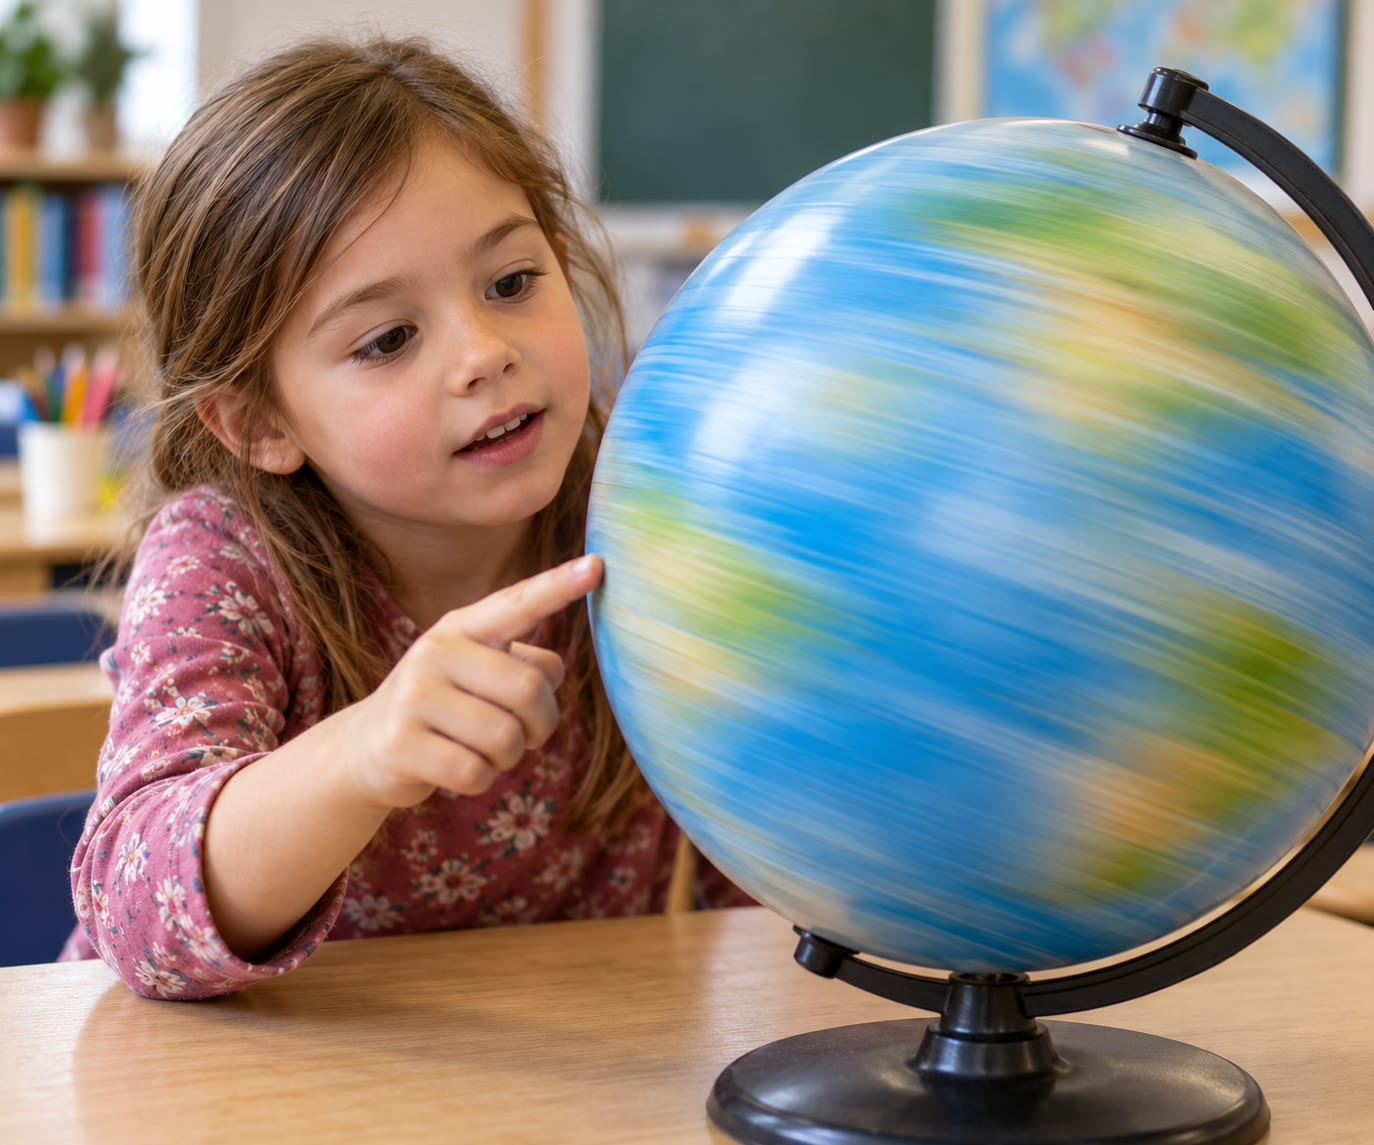
\includegraphics[width=0.6\linewidth]{images/book1/ai/g3-spinning-globe.jpg}

{\small \omterm{def:g3:continents-and-oceans:globe}{مجسم للكرة الأرضية} يدور على حامله: اليابسة \omterm{def:g2:water-on-earth:ocean}{والبحر} يمران تحت
الإصبع.}
\end{omfigure}

\begin{recall}
معظم الأرض يغطيه \omterm{def:g2:water-on-earth:salt-fresh}{الماء المالح}: نحو 71 مربعًا من كل 100 في شبكة
\cref{ch:g2:water-on-earth}. \omterm{def:g2:water-on-earth:ocean}{والمحيط} مساحة واسعة جدًا من \omterm{def:g2:water-on-earth:salt-fresh}{الماء المالح}
بين كتل اليابسة؛ \omterm{def:g2:water-on-earth:ocean}{والبحر} مساحة أصغر، على طرف \omterm{def:g2:water-on-earth:ocean}{محيط}. \omterm{def:g2:drawing-to-map:map}{والخريطة} رسم لمكان كما
يُرى من الأعلى، مصغَّرًا (\cref{ch:g2:drawing-to-map}). وكتب الفيزياء
تحكي كيف تدور الأرض حول نفسها مرة كل يوم، فيكون لنا النهار والليل.
\end{recall}

\section{مجسم الكرة الأرضية، نموذج صغير للأرض المستديرة}

الأرض مستديرة، مثل كرة كبيرة جدًا. ولا نستطيع أن نرى شكلها من سطحها،
لأنها أكبر من ذلك بكثير: فأينما وقفنا تبدو الأرض مستوية. لكن رواد
الفضاء الذين سافروا بعيدًا عن الأرض رأوها كاملة، كرة زرقاء مستديرة في
السماء السوداء (الصورة في أول
\cref{ch:g2:water-on-earth}).

لكي نرى الأرض كلها في غرفة الصف، نصغّرها.

\begin{definition}[مجسم الكرة الأرضية]\label{def:g3:continents-and-oceans:globe}
\emph{مجسم الكرة الأرضية}\index{مجسم الكرة الأرضية} نموذج للأرض: كرة
رُسمت عليها اليابسة والمحيطات بأشكالها نفسها على الأرض الحقيقية،
لكنها أصغر بكثير جدًا.
\end{definition}

\omterm{def:g3:continents-and-oceans:globe}{مجسم الكرة الأرضية} أفضل صورة للأرض، لأن له الشكل الصحيح: مستدير. لكننا،
كما في الأرض الحقيقية، لا نرى منه إلا نصفه في كل مرة. ولكي نرى النصف
الآخر، ندير \omterm{def:g3:continents-and-oceans:globe}{المجسم}.

\begin{omfigure}
\begin{tikzpicture}
\begin{axis}[name=atl, hide axis, axis equal image, scale only axis,
    width=6.2cm, xmin=-1.05, xmax=1.05, ymin=-1.05, ymax=1.05, clip=false]
  \fill[omSea] (axis cs:0,0) circle[radius=1];
  \addplot[fill=omHypsLandA!85!black, draw=black!45, line width=0.2pt]
    table {figdata/out/grade-3-globe-atlantic-land.dat};
  \addplot[black!60, dashed, line width=0.5pt]
    table {figdata/out/grade-3-globe-atlantic-equator.dat};
  \addplot[only marks, mark=*, mark size=1.4pt, black]
    table[x=x, y=y] {figdata/out/grade-3-globe-atlantic-poles.dat};
  \node[font=\scriptsize, anchor=center, align=center, fill=white, fill opacity=0.7, text opacity=1, inner sep=1pt, rounded corners=1pt] at (axis cs:-0.683,0.636) {أمريكا\\الشمالية};
  \node[font=\scriptsize, anchor=center, align=center, fill=white, fill opacity=0.7, text opacity=1, inner sep=1pt, rounded corners=1pt] at (axis cs:-0.561,-0.408) {أمريكا\\الجنوبية};
  \node[font=\scriptsize, anchor=center, align=center, fill=white, fill opacity=0.7, text opacity=1, inner sep=1pt, rounded corners=1pt] at (axis cs:0.396,0.639) {أوروبا};
  \node[font=\scriptsize, anchor=center, align=center, fill=white, fill opacity=0.7, text opacity=1, inner sep=1pt, rounded corners=1pt] at (axis cs:0.704,-0.098) {إفريقيا};
  \node[font=\scriptsize, anchor=center, align=center, fill=white, fill opacity=0.7, text opacity=1, inner sep=1pt, rounded corners=1pt] at (axis cs:-0.209,0.128) {المحيط\\الأطلسي};
  \draw[black!70, line width=0.8pt] (axis cs:0,0) circle[radius=1];
  \node[font=\scriptsize, anchor=south] at (axis cs:0,0.97) {القطب الشمالي};
\end{axis}
\begin{axis}[at={(atl.east)}, anchor=west, xshift=0.6cm, hide axis,
    axis equal image, scale only axis,
    width=6.2cm, xmin=-1.05, xmax=1.05, ymin=-1.05, ymax=1.05, clip=false]
  \fill[omSea] (axis cs:0,0) circle[radius=1];
  \addplot[fill=omHypsLandA!85!black, draw=black!45, line width=0.2pt]
    table {figdata/out/grade-3-globe-pacific-land.dat};
  \addplot[black!60, dashed, line width=0.5pt]
    table {figdata/out/grade-3-globe-pacific-equator.dat};
  \node[font=\scriptsize, anchor=center, align=center, fill=white, fill opacity=0.7, text opacity=1, inner sep=1pt, rounded corners=1pt] at (axis cs:-0.754,-0.391) {أستراليا};
  \node[font=\scriptsize, anchor=center, align=center, fill=white, fill opacity=0.7, text opacity=1, inner sep=1pt, rounded corners=1pt] at (axis cs:0.258,0.087) {المحيط\\الهادئ};
  \draw[black!70, line width=0.8pt] (axis cs:0,0) circle[radius=1];
\end{axis}
\end{tikzpicture}

{\small \omterm{def:g3:continents-and-oceans:globe}{مجسم الكرة الأرضية} من جهتين. يسارًا: جهة \omterm{def:g2:water-on-earth:ocean}{المحيط} الأطلسي، وفيها
الأمريكتان وأوروبا وإفريقيا. يمينًا: الجهة الأخرى، جهة \omterm{def:g2:water-on-earth:ocean}{المحيط} الهادئ،
وأستراليا على طرفه. الخط المتقطع هو \omterm{def:g3:continents-and-oceans:equator}{خط الاستواء}.
خطوط السواحل: Natural Earth (ملك عام).}
\label{fig:g3:continents-and-oceans:globes}
% ledger: data:ne-land
\end{omfigure}

\begin{remark}[نصفان مختلفان جدًا]\label{rem:g3:continents-and-oceans:halves}
انظر إلى الصورتين. في اليسرى، تغطي اليابسة نحو 4 أجزاء من الصورة من كل
10. وفي اليمنى، نحو جزء واحد فقط من كل 10: فجهة \omterm{def:g2:water-on-earth:ocean}{المحيط} الهادئ من الأرض
كلها تقريبًا ماء. وإذا وقفت إصبع لينا على تلك الجهة من \omterm{def:g3:continents-and-oceans:globe}{المجسم}، فستقع على
\omterm{def:g2:water-on-earth:ocean}{البحر} في كل مرة تقريبًا.
\end{remark}

\section{خط الاستواء والقطبان ونصفا الكرة}

يدور \omterm{def:g3:continents-and-oceans:globe}{مجسم الكرة الأرضية} حول قضيب يخترقه من أعلاه إلى أسفله. والأرض
الحقيقية ليس لها قضيب، لكنها تدور هي أيضًا حول خط يمر بوسطها. وللمكانين
اللذين يخرج منهما ذلك الخط من الأرض اسمان.

\begin{definition}[القطب]\label{def:g3:continents-and-oceans:poles}
\emph{القطب الشمالي}\index{القطب الشمالي} و\emph{القطب
الجنوبي}\index{القطب الجنوبي} هما النقطتان في أعلى الأرض تمامًا وأسفلها
تمامًا، حيث يخرج الخط الذي تدور حوله الأرض. وكل واحدة منهما
\emph{قطب}\index{قطب}. وفي \omterm{def:g3:continents-and-oceans:globe}{مجسم الكرة الأرضية} يكون القطب الشمالي في
الأعلى.
\end{definition}

\begin{definition}[خط الاستواء ونصف الكرة]\label{def:g3:continents-and-oceans:equator}
\emph{خط الاستواء}\index{خط الاستواء} خط وهمي مرسوم حول الأرض كلها، في
منتصف المسافة تمامًا بين \omterm{def:g3:continents-and-oceans:poles}{القطب الشمالي} \omterm{def:g3:continents-and-oceans:poles}{والقطب الجنوبي}. إنه يقسم الأرض
إلى نصفين، يسمى كل منهما
\emph{نصف الكرة}\index{نصف الكرة}: \emph{نصف الكرة
الشمالي}\index{نصف الكرة الشمالي}، في جهة \omterm{def:g3:continents-and-oceans:poles}{القطب الشمالي}، و\emph{نصف
الكرة الجنوبي}\index{نصف الكرة الجنوبي}، في جهة
\omterm{def:g3:continents-and-oceans:poles}{القطب الجنوبي}.
\end{definition}

\omterm{def:g3:continents-and-oceans:equator}{خط الاستواء} ليس مرسومًا على الأرض: لا يستطيع أحد أن يراه على شاطئ أو في
غابة. إنه يُرسم على \omterm{def:g3:continents-and-oceans:globe}{مجسمات الكرة الأرضية} وعلى الخرائط ليساعدنا على الاهتداء.

\begin{omfigure}
\begin{tikzpicture}[font=\small]
  % globe outline
  \fill[omSea!70] (0,0) circle (2.2);
  % northern hemisphere tinted
  \begin{scope}
    \clip (0,0) circle (2.2);
    \fill[yellow!25, opacity=0.8] (-2.3,0) -- (-2.3,2.3) -- (2.3,2.3) -- (2.3,0)
      arc[start angle=0, end angle=-180, x radius=2.3, y radius=0.45] -- cycle;
  \end{scope}
  \draw[black!70, line width=0.8pt] (0,0) circle (2.2);
  % equator: front half solid, back half dashed
  \draw[red!70!black, line width=1.2pt] (-2.2,0) arc[start angle=180, end angle=360, x radius=2.2, y radius=0.4];
  \draw[red!70!black, line width=0.8pt, dashed] (2.2,0) arc[start angle=0, end angle=180, x radius=2.2, y radius=0.4];
  % axis and poles
  \draw[black!60, line width=0.6pt] (0,2.2) -- (0,2.75);
  \draw[black!60, line width=0.6pt] (0,-2.2) -- (0,-2.75);
  \draw[black!60, line width=0.6pt, dotted] (0,2.2) -- (0,-2.2);
  \fill (0,2.2) circle (2.2pt);
  \fill (0,-2.2) circle (2.2pt);
  \node[anchor=west] at (0.15,2.6) {القطب الشمالي};
  \node[anchor=west] at (0.15,-2.6) {القطب الجنوبي};
  % labels
  \node[anchor=west] at (2.6,0) {خط الاستواء};
  \draw[black!60] (2.55,0) -- (2.05,-0.15);
  \node[anchor=west, align=left] at (2.6,1.4) {نصف الكرة\\الشمالي};
  \draw[black!60] (2.55,1.4) -- (1.5,1.2);
  \node[anchor=west, align=left] at (2.6,-1.4) {نصف الكرة\\الجنوبي};
  \draw[black!60] (2.55,-1.4) -- (1.5,-1.2);
\end{tikzpicture}

{\small \omterm{def:g3:continents-and-oceans:equator}{خط الاستواء} يقسم الأرض إلى نصفي كرة. \omterm{def:g3:continents-and-oceans:equator}{نصف الكرة الشمالي} (الملوّن)
في جهة \omterm{def:g3:continents-and-oceans:poles}{القطب الشمالي}، \omterm{def:g3:continents-and-oceans:equator}{ونصف الكرة الجنوبي} في جهة
\omterm{def:g3:continents-and-oceans:poles}{القطب الجنوبي}.}
\label{fig:g3:continents-and-oceans:hemispheres}
\end{omfigure}

\begin{example}[حر قرب خط الاستواء، وبرد قرب القطبين]\label{ex:g3:continents-and-oceans:hot-cold}
الأراضي القريبة من \omterm{def:g3:continents-and-oceans:equator}{خط الاستواء} حارة طوال السنة: هناك تنمو الغابات المطيرة
العظيمة. والأراضي القريبة من \omterm{def:g3:continents-and-oceans:poles}{القطبين} باردة طوال السنة، ويغطي الجليد
جزءًا كبيرًا منها. وستتعلم في سنة لاحقة لماذا هي كذلك؛ أما الآن فتذكر:
كلما اقتربنا من \omterm{def:g3:continents-and-oceans:poles}{قطب}، اشتد البرد.
\end{example}

\section{سبع قارات وخمسة محيطات}

على \omterm{def:g3:continents-and-oceans:globe}{مجسم الكرة الأرضية}، لا تنتشر اليابسة قطعًا صغيرة في كل مكان. بل يتجمع
معظمها في بضع كتل واسعة جدًا.

\begin{definition}[القارة]\label{def:g3:continents-and-oceans:continent}
\emph{القارة}\index{قارة} واحدة من كتل اليابسة الواسعة جدًا على الأرض،
مع الجزر القريبة منها.
\end{definition}

يعدّ الناس في الغالب سبع \omterm{def:g3:continents-and-oceans:continent}{قارات}. وهي من الأكبر إلى الأصغر: آسيا،
وإفريقيا، وأمريكا الشمالية، وأمريكا الجنوبية، والقارة القطبية الجنوبية،
وأوروبا، وأستراليا.
% ledger: natgeo:seven-continents

\begin{center}\small
\begin{tabular}{rlll}
\hline
الترتيب & \omterm{def:g3:continents-and-oceans:continent}{القارة} & \omterm{def:g3:continents-and-oceans:equator}{نصف الكرة} & كلمة عنها \\
\hline
1 & آسيا & الشمالي في أغلبها & الأكبر \\
2 & إفريقيا & كلاهما & \omterm{def:g3:continents-and-oceans:equator}{خط الاستواء} يعبر وسطها \\
3 & أمريكا الشمالية & الشمالي & تمتد بعيدًا نحو الشمال \\
4 & أمريكا الجنوبية & الجنوبي في أغلبها & \omterm{def:g3:continents-and-oceans:equator}{خط الاستواء} يعبر شمالها \\
5 & القارة القطبية الجنوبية & الجنوبي & حول \omterm{def:g3:continents-and-oceans:poles}{القطب الجنوبي}، تحت الجليد \\
6 & أوروبا & الشمالي & متصلة بآسيا من جهتها الشرقية \\
7 & أستراليا & الجنوبي & الأصغر \\
\hline
\end{tabular}
\end{center}

\begin{remark}[أين تنتهي القارة؟]\label{rem:g3:continents-and-oceans:where}
بعض \omterm{def:g3:continents-and-oceans:continent}{القارات} يحيط بها \omterm{def:g2:water-on-earth:ocean}{البحر} من كل جانب، مثل أستراليا أو القارة القطبية
الجنوبية. وبعضها متلاصق: فأوروبا وآسيا كتلة واحدة من اليابسة، والناس هم
الذين اختاروا أين يرسمون الحد بينهما. لذلك يعدّ بعض الناس ست \omterm{def:g3:continents-and-oceans:continent}{قارات}، أو
أقل.
\end{remark}

بين \omterm{def:g3:continents-and-oceans:continent}{القارات} تمتد المحيطات. وعددها خمسة. أكبرها
\emph{\omterm{def:g2:water-on-earth:ocean}{المحيط} الهادئ}؛ ثم يأتي \emph{\omterm{def:g2:water-on-earth:ocean}{المحيط} الأطلسي}، ثم
\emph{\omterm{def:g2:water-on-earth:ocean}{المحيط} الهندي}، ثم \emph{\omterm{def:g2:water-on-earth:ocean}{المحيط} الجنوبي} حول القارة القطبية الجنوبية،
وأصغرها \emph{\omterm{def:g2:water-on-earth:ocean}{المحيط} المتجمد الشمالي} حول \omterm{def:g3:continents-and-oceans:poles}{القطب الشمالي}. وظل الناس زمنًا
طويلًا يعدّون أربعة فقط؛ واليوم تعدّ أكثر البلدان \omterm{def:g2:water-on-earth:ocean}{المحيط} الجنوبي
خامسها.
% ledger: nos:five-oceans, nos:pacific-largest, oer:arctic-smallest

\begin{example}[ما مقدار اتساع المحيط الهادئ؟]\label{ex:g3:continents-and-oceans:pacific}
\omterm{def:g2:water-on-earth:ocean}{المحيط} الهادئ واسع جدًا حتى إن \omterm{def:g3:continents-and-oceans:continent}{القارات} كلها مجتمعة تتسع داخله. وهو يحوي
أكثر من نصف ماء المحيطات كله على الأرض. لذلك يبدو \omterm{def:g3:continents-and-oceans:globe}{المجسم} الأيمن في القسم
الأول من هذا الفصل أزرق كله
تقريبًا.
% ledger: nos:pacific-largest
\end{example}

\begin{method}[تسمية المحيط الذي بين قارتين]\label{met:g3:continents-and-oceans:between}
لتعرف أي \omterm{def:g2:water-on-earth:ocean}{محيط} يقع بين قارتين، ضع إصبعًا على كل منهما على \omterm{def:g3:continents-and-oceans:globe}{مجسم الكرة
الأرضية}، وأدر \omterm{def:g3:continents-and-oceans:globe}{المجسم} حتى ترى الاثنتين. \omterm{def:g2:water-on-earth:ocean}{المحيط} الذي تعبره عينك من إصبع
إلى الأخرى هو الذي بينهما.
وعلى \omterm{def:g3:continents-and-oceans:globe}{المجسم} يوجد في الغالب طريقان للالتفاف: خذ الأقصر.
\end{method}

\begin{example}[إفريقيا وأستراليا]\label{ex:g3:continents-and-oceans:africa-australia}
إذا ذهبنا من إفريقيا شرقًا نحو أستراليا عبرنا \omterm{def:g2:water-on-earth:ocean}{المحيط} الهندي. وإذا ذهبنا من
أوروبا غربًا إلى أمريكا الشمالية عبرنا \omterm{def:g2:water-on-earth:ocean}{المحيط} الأطلسي. وإذا ذهبنا من آسيا
شرقًا إلى أمريكا الشمالية عبرنا \omterm{def:g2:water-on-earth:ocean}{المحيط} الهادئ.
\end{example}

\section{خريطة العالم مجسمٌ مبسوط}

\omterm{def:g3:continents-and-oceans:globe}{مجسم الكرة الأرضية} مستدير، فليس من السهل حمله، ولا نستطيع أبدًا أن نراه
كله دفعة واحدة. أما \omterm{def:g2:drawing-to-map:map}{الخريطة} على ورقة فتبين الأرض كلها بنظرة واحدة.

\begin{definition}[خريطة العالم]\label{def:g3:continents-and-oceans:world-map}
\emph{خريطة العالم}\index{خريطة العالم} \omterm{def:g2:drawing-to-map:map}{خريطة} للأرض كلها مرسومة مسطحة
على ورقة أو على شاشة، فيها كل \omterm{def:g3:continents-and-oceans:continent}{القارات} وكل المحيطات في صورة
واحدة.
\end{definition}

\begin{omfigure}
\begin{tikzpicture}
\begin{axis}[ommap, width=\linewidth, xtick=\empty, ytick={0},
    yticklabels={خط الاستواء}, grid=none, clip=true]
  \addplot[fill=omHypsLandA!85!black, draw=black!45, line width=0.2pt]
    table {figdata/out/shared-geo-land.dat};
  \draw[black!60, dashed, line width=0.5pt] (axis cs:-180,0) -- (axis cs:180,0);
  \begin{scope}[every node/.style={font=\scriptsize, align=center}]
    \node at (axis cs:-102,47) {أمريكا\\الشمالية};
    \node at (axis cs:-60,-12) {أمريكا\\الجنوبية};
    \node at (axis cs:17,52) {أوروبا};
    \node at (axis cs:20,6) {إفريقيا};
    \node at (axis cs:92,48) {آسيا};
    \node at (axis cs:134,-24) {أستراليا};
    \node at (axis cs:40,-80) {القارة القطبية الجنوبية};
  \end{scope}
  \begin{scope}[every node/.style={font=\scriptsize\itshape, align=center, text=omSea!35!black}]
    \node at (axis cs:-145,8) {المحيط\\الهادئ};
    \node at (axis cs:165,12) {المحيط\\الهادئ};
    \node at (axis cs:-38,22) {المحيط\\الأطلسي};
    \node at (axis cs:-15,-25) {المحيط\\الأطلسي};
    \node at (axis cs:78,-22) {المحيط\\الهندي};
    \node at (axis cs:-115,-57) {المحيط الجنوبي};
    \node at (axis cs:-150,79) {المحيط المتجمد الشمالي};
  \end{scope}
\end{axis}
\end{tikzpicture}

{\small \omterm{def:g3:continents-and-oceans:world-map}{خريطة العالم}. قُطع \omterm{def:g3:continents-and-oceans:globe}{مجسم الكرة الأرضية} على طول خط يمر بوسط \omterm{def:g2:water-on-earth:ocean}{المحيط}
الهادئ ثم بُسط: لذلك يظهر \omterm{def:g2:water-on-earth:ocean}{المحيط} الهادئ مرتين، على الطرف الأيسر وعلى
الطرف الأيمن. والقارة القطبية الجنوبية، وهي \omterm{def:g3:continents-and-oceans:continent}{قارة} مستديرة حول \omterm{def:g3:continents-and-oceans:poles}{القطب
الجنوبي}، تمددت فصارت شريطًا طويلًا على طول الأسفل.
خطوط السواحل: Natural Earth (ملك عام).}
\label{fig:g3:continents-and-oceans:world-map}
% ledger: data:ne-land
\end{omfigure}

لكن هناك صعوبة. حاول أن تبسط قشرة برتقالة على طاولة: لا تستطيع أن تستوي
دون أن تتمزق أو تتمدد. والأمر نفسه يحدث لسطح \omterm{def:g3:continents-and-oceans:globe}{مجسم الكرة الأرضية} حين
يُرسم مسطحًا. فكل \omterm{def:g3:continents-and-oceans:world-map}{خريطة للعالم} تمزق \omterm{def:g3:continents-and-oceans:globe}{المجسم} في مكان ما، أو تمدد بعض
الأماكن وتضغط غيرها.

\begin{omfigure}
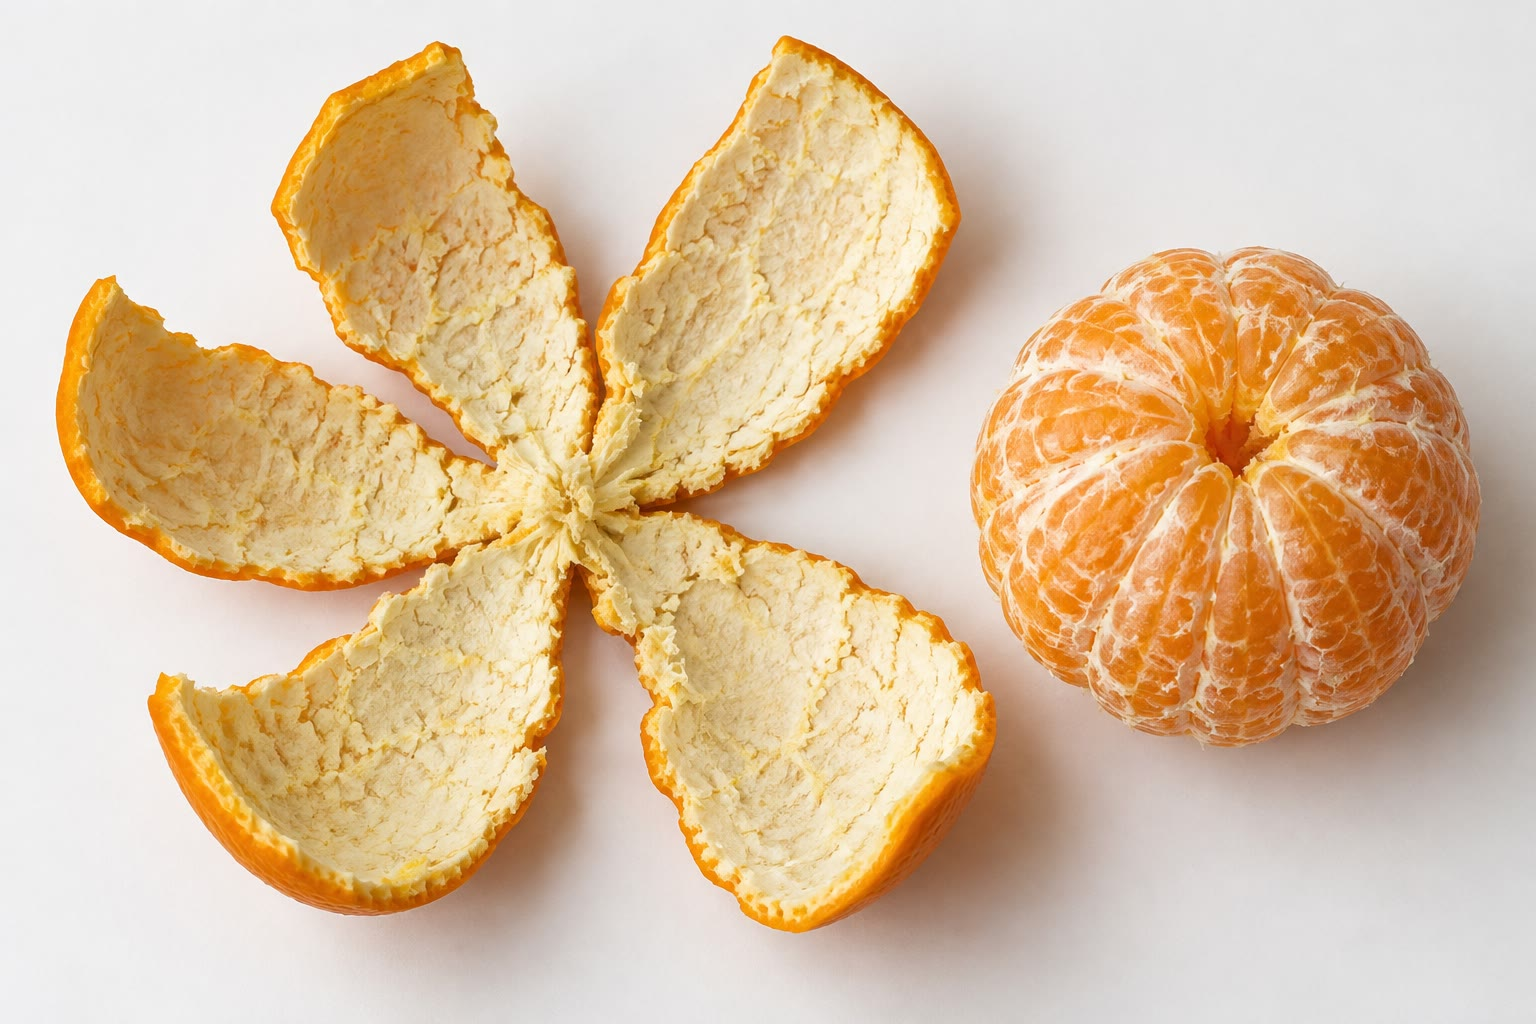
\includegraphics[width=0.4\linewidth]{images/book1/ai/g3-orange-peel.jpg}

{\small قشرة البرتقالة لا تستوي على سطح مستوٍ دون أن تتمزق.}
\end{omfigure}

\begin{remark}[الخريطة والمجسم لا يتفقان]\label{rem:g3:continents-and-oceans:disagree}
في \omterm{def:g3:continents-and-oceans:world-map}{خريطة العالم} هذه تبدو القارة القطبية الجنوبية من أكبر \omterm{def:g3:continents-and-oceans:continent}{القارات}، ممدودة
على طول الحافة السفلى كلها. أما على \omterm{def:g3:continents-and-oceans:globe}{المجسم} فهي كتلة مستديرة من اليابسة،
أصغر من أمريكا الجنوبية. فقرب \omterm{def:g3:continents-and-oceans:poles}{القطبين} تمدد \omterm{def:g2:drawing-to-map:map}{الخريطة} المسطحة اليابسة كثيرًا،
وقرب \omterm{def:g3:continents-and-oceans:equator}{خط الاستواء} تمددها قليلًا جدًا. وحين تريد أن تقارن مساحة مكانين بعيدين
عن \omterm{def:g3:continents-and-oceans:equator}{خط الاستواء}، \omterm{def:g3:continents-and-oceans:globe}{فالمجسم} هو الذي يقول
الحقيقة.
\end{remark}

\begin{method}[قراءة خريطة العالم]\label{met:g3:continents-and-oceans:reading}
في \omterm{def:g3:continents-and-oceans:world-map}{خريطة للعالم} مثل هذه:
\begin{enumerate}
  \item الشمال في الأعلى، والجنوب في الأسفل؛ \omterm{def:g3:continents-and-oceans:poles}{والقطب الشمالي} هو الحافة
        العليا كلها، \omterm{def:g3:continents-and-oceans:poles}{والقطب الجنوبي} الحافة السفلى كلها؛
  \item \omterm{def:g3:continents-and-oceans:equator}{خط الاستواء} هو الخط الذي يعبر الوسط: كل ما فوقه في \omterm{def:g3:continents-and-oceans:equator}{نصف الكرة
        الشمالي}، وكل ما تحته في \omterm{def:g3:continents-and-oceans:equator}{نصف الكرة
        الجنوبي}؛
  \item الحافتان اليسرى واليمنى هما الخط نفسه على \omterm{def:g3:continents-and-oceans:globe}{المجسم}: السفينة التي
        تخرج من الحافة اليمنى تعود من اليسرى.
\end{enumerate}
\end{method}

\section{تمارين}

\begin{exercise}[$\star$]\label{exo:g3:continents-and-oceans:1}
سمِّ \omterm{def:g3:continents-and-oceans:continent}{القارات} السبع. أيها الأكبر؟ وأيها الأصغر؟
\end{exercise}

\begin{exercise}[$\star$]\label{exo:g3:continents-and-oceans:2}
سمِّ المحيطات الخمسة. أيها الأكبر؟ وأيها الأصغر؟
\end{exercise}

\begin{exercise}[$\star$]\label{exo:g3:continents-and-oceans:3}
انقل وأكمل بإحدى العبارات «\omterm{def:g3:continents-and-oceans:poles}{القطب الشمالي}» أو «\omterm{def:g3:continents-and-oceans:poles}{القطب الجنوبي}» أو «\omterm{def:g3:continents-and-oceans:equator}{خط الاستواء}»: \dots{}
في أعلى \omterm{def:g3:continents-and-oceans:globe}{مجسم الكرة الأرضية}؛ و\dots{} في أسفله؛ و\dots{}
يدور حول وسطه كله.
\end{exercise}

\begin{exercise}[$\star$]\label{exo:g3:continents-and-oceans:4}
\omterm{def:g3:continents-and-oceans:equator}{نصف الكرة الشمالي} أم الجنوبي؟ أوروبا؛ أستراليا؛ القارة القطبية الجنوبية؛
أمريكا الشمالية.
\end{exercise}

\begin{exercise}[$\star$]\label{exo:g3:continents-and-oceans:5}
أي \omterm{def:g2:water-on-earth:ocean}{محيط} يقع حول \omterm{def:g3:continents-and-oceans:poles}{القطب الشمالي}؟ وأي \omterm{def:g2:water-on-earth:ocean}{محيط} يقع حول
القارة القطبية الجنوبية؟
\end{exercise}

\begin{exercise}[$\star\star$]\label{exo:g3:continents-and-oceans:6}
أي \omterm{def:g2:water-on-earth:ocean}{محيط} تعبر لتذهب من إفريقيا إلى أمريكا الجنوبية؟ ومن
أستراليا إلى أمريكا الجنوبية، متجهًا شرقًا؟ ومن إفريقيا إلى أستراليا؟
\end{exercise}

\begin{exercise}[$\star\star$]\label{exo:g3:continents-and-oceans:7}
يعيش سام في بلد حار طوال السنة. ويعيش بو في محطة أبحاث يشتد فيها البرد
طوال السنة. أحدهما يعيش قرب \omterm{def:g3:continents-and-oceans:equator}{خط الاستواء}، والآخر قرب \omterm{def:g3:continents-and-oceans:poles}{قطب}. من يعيش
أين؟
\end{exercise}

\begin{exercise}[$\star\star$]\label{exo:g3:continents-and-oceans:8}
تدير لينا \omterm{def:g3:continents-and-oceans:globe}{مجسم الكرة الأرضية} 10 مرات. فيقع إصبعها على \omterm{def:g2:water-on-earth:ocean}{البحر} 7 مرات. كم
مرة يقع على اليابسة؟ أهذا ما كنت تتوقعه؟ لماذا؟
\end{exercise}

\begin{exercise}[$\star\star$]\label{exo:g3:continents-and-oceans:9}
في \omterm{def:g3:continents-and-oceans:world-map}{خريطة العالم} في الصفحة~\pageref{fig:g3:continents-and-oceans:world-map}،
يظهر \omterm{def:g2:water-on-earth:ocean}{المحيط} الهادئ مرتين. لماذا؟ أللأرض الحقيقية محيطان
هادئان؟
\end{exercise}

\begin{exercise}[$\star\star\star$]\label{exo:g3:continents-and-oceans:10}
يقول توم: «على \omterm{def:g3:continents-and-oceans:world-map}{خريطة العالم}، القارة القطبية الجنوبية أطول من آسيا، إذن هي
أكبر \omterm{def:g3:continents-and-oceans:continent}{القارات}.» هل توم محق؟ استعمل قائمة \omterm{def:g3:continents-and-oceans:continent}{القارات}
من الأكبر إلى الأصغر، وقل لماذا تخدعه \omterm{def:g3:continents-and-oceans:world-map}{خريطة العالم}.
\end{exercise}
